%==============================================================================
%  Partie 1 : automatisation de l'infrastructure
%  Etat d'avancement : Terraform et Ansible
%  Compilation : latexmk -pdf Partie1-Automatisation.tex
%==============================================================================
\documentclass[11pt,a4paper]{article}

\usepackage[utf8]{inputenc}
\usepackage[T1]{fontenc}
\usepackage[french]{babel}
\usepackage{newtxtext,newtxmath}
\usepackage{microtype}

\usepackage[a4paper,top=2.2cm,bottom=2.0cm,left=2.0cm,right=2.0cm,headheight=14pt]{geometry}
\usepackage{fancyhdr}
\usepackage{titlesec}
\usepackage{lastpage}
\usepackage{setspace}
\setstretch{1.02}

\usepackage{array}
\usepackage{tabularx}
\usepackage{booktabs}
\usepackage{colortbl}
\usepackage{ragged2e}
\usepackage{enumitem}
\usepackage{float}
\usepackage{caption}
\usepackage{graphicx}
\usepackage{xcolor}
\usepackage[most]{tcolorbox}
\usepackage{etoolbox}
\usepackage{needspace}

\definecolor{primary}{HTML}{00205B}
\definecolor{accent}{HTML}{0F7FA5}
\definecolor{soft}{HTML}{E8EEF5}
\definecolor{warn}{HTML}{B3541E}
\definecolor{okgreen}{HTML}{1F7A4D}
\definecolor{gris}{HTML}{5A5A5A}

\usepackage[hidelinks]{hyperref}
\hypersetup{colorlinks=true, linkcolor=primary, urlcolor=accent,
  pdftitle={Partie 1 - Automatisation de l'infrastructure},
  pdfauthor={Stage Airbus - Infrastructure et Securite Reseau}}

\titleformat{\section}{\normalfont\large\sffamily\bfseries\color{primary}}{\thesection.}{0.6em}{}
\titlespacing*{\section}{0pt}{13pt}{6pt}
\titleformat{\subsection}{\normalfont\normalsize\sffamily\bfseries\color{accent!85!black}}{\thesubsection}{0.6em}{}
\titlespacing*{\subsection}{0pt}{9pt}{4pt}

\pagestyle{fancy}
\fancyhf{}
\renewcommand{\headrulewidth}{0.4pt}
\renewcommand{\footrulewidth}{0.4pt}
\fancyhead[L]{\footnotesize\textcolor{primary}{\textbf{Partie 1 : automatisation de l'infrastructure}}}
\fancyhead[R]{\footnotesize\textcolor{gris}{\rightmark}}
\fancyfoot[L]{\footnotesize\textcolor{gris}{Airbus, diffusion interne}}
\fancyfoot[R]{\footnotesize\textcolor{gris}{Page \thepage\ / \pageref{LastPage}}}
\renewcommand{\sectionmark}[1]{\markright{\thesection.~#1}}

\newcolumntype{Y}{>{\RaggedRight\arraybackslash}X}
\newcolumntype{L}[1]{>{\RaggedRight\arraybackslash}p{#1}}
\newcolumntype{C}[1]{>{\Centering\arraybackslash}p{#1}}

\captionsetup{font=small,labelfont={bf,color=primary},skip=5pt,labelsep=period}
\addto\captionsfrench{\renewcommand{\tablename}{Tableau}}
\renewcommand{\arraystretch}{1.08}
\AtBeginEnvironment{tabularx}{\small}
\AtBeginDocument{\setlist[itemize,1]{label=\textbullet}}

\pretocmd{\section}{\needspace{10\baselineskip}}{}{}
\pretocmd{\subsection}{\needspace{5\baselineskip}}{}{}

\newtcolorbox{notebox}[1][Note technique]{
  enhanced, breakable, colback=soft, colframe=primary,
  boxrule=0.7pt, arc=2pt, left=6pt, right=6pt, top=4pt, bottom=4pt,
  fonttitle=\bfseries\sffamily\small, title={#1}, coltitle=white}

\newtcolorbox{alertbox}[1][Point de vigilance]{
  enhanced, breakable, colback=warn!6, colframe=warn,
  boxrule=0.7pt, arc=2pt, left=6pt, right=6pt, top=4pt, bottom=4pt,
  fonttitle=\bfseries\sffamily\small, title={#1}, coltitle=white}

\newcommand{\ttb}[1]{\texttt{\small #1}}
\newcommand{\rid}[1]{\textcolor{primary}{\textbf{\small #1}}}
\newcommand{\ok}{\textcolor{okgreen}{\textbf{Conforme}}}

\begin{document}

%------------------------------------------------------------------ en-tete
\begin{center}
{\sffamily\Large\bfseries\color{primary} AIRBUS}\\[2pt]
{\sffamily\footnotesize\color{gris} Direction des Systèmes d'Information, Infrastructure et Sécurité Réseau}

\vspace{10pt}
\noindent\textcolor{primary}{\rule{\textwidth}{2.5pt}}\\[10pt]
{\sffamily\huge\bfseries\color{primary} Partie 1 : automatisation\\[4pt] de l'infrastructure}\\[8pt]
{\sffamily\normalsize\itshape\color{gris} État d'avancement : Terraform et Ansible}\\[8pt]
\noindent\textcolor{accent}{\rule{\textwidth}{1pt}}
\end{center}

\vspace{6pt}

\begin{notebox}[En deux mots]
La partie 1 du cahier des charges est désormais automatisée de bout en bout.
\textbf{Terraform} crée les six machines et les sept réseaux du laboratoire.
\textbf{Ansible} installe et configure les services métiers, la supervision et les
deux pare-feux. L'ensemble est rejouable : détruire puis reconstruire le
laboratoire redonne exactement la même infrastructure, avec la même
configuration, sans intervention manuelle.
\end{notebox}

%==============================================================================
\section{Vue d'ensemble}
%==============================================================================

Le projet s'appuie sur trois outils, chacun avec un périmètre précis. Ce
découpage n'est pas cosmétique : il découle d'une limite technique de
cloud-init, qui ne s'exécute qu'une seule fois, au premier démarrage de la
machine.

\begin{figure}[H]
\centering
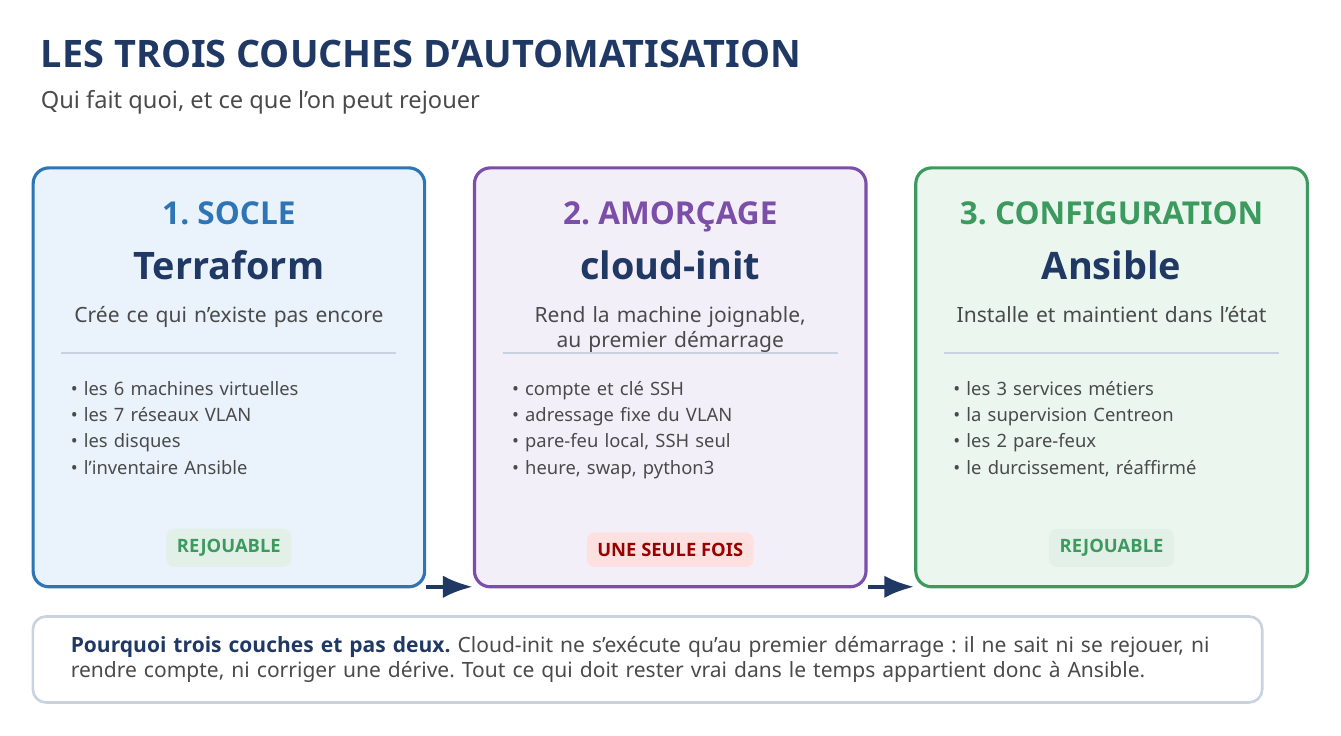
\includegraphics[width=\textwidth]{figures/figure1-couches.png}
\caption{Les trois couches d'automatisation}
\end{figure}

Une première version confiait l'installation des services à cloud-init. Cette
approche a été abandonnée : cloud-init ne sait ni se rejouer, ni rendre compte
de ce qu'il a fait, ni corriger une configuration qui aurait dérivé. La moindre
modification obligerait à détruire puis recréer la machine. Il a donc été ramené
à son seul rôle d'amorçage.

\begin{table}[H]
\centering
\caption{Volumétrie du projet}
\begin{tabularx}{\textwidth}{L{3.2cm} C{2.6cm} C{2.6cm} Y}
\toprule
\rowcolor{soft}\textbf{Couche} & \textbf{Lignes} & \textbf{Unités} & \textbf{Contenu} \\
\midrule
Terraform & 1 100 & 3 modules & \ttb{reseau}, \ttb{serveur}, \ttb{parefeu} \\
Ansible & 1 500 & 7 rôles & 84 tâches réparties par service \\
\midrule
\textbf{Total} & \textbf{2 600} & & Commentaires : 6 \% du code \\
\bottomrule
\end{tabularx}
\end{table}

%==============================================================================
\section{Terraform : le socle}
%==============================================================================

La cible retenue est KVM et libvirt, ce qui correspond au scénario B du cahier
des charges : une virtualisation locale, sans cloud public. C'est cette
architecture qui sera déployée sur la machine Intel fournie par l'entreprise.

\begin{figure}[H]
\centering
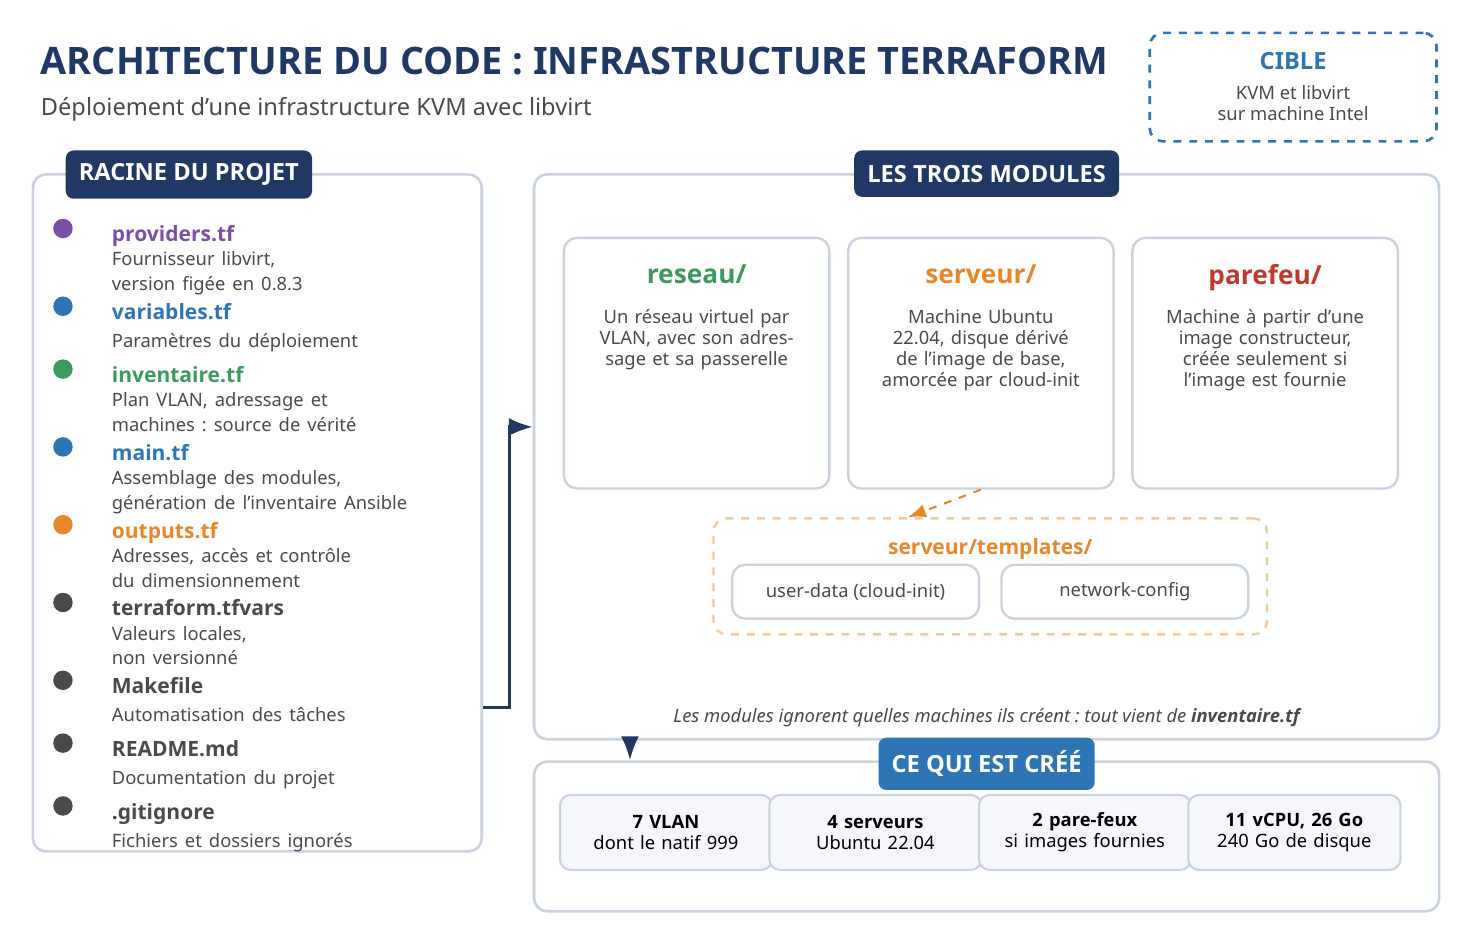
\includegraphics[width=\textwidth]{figures/figure2-terraform.png}
\caption{Architecture du code : infrastructure Terraform}
\end{figure}

\subsection{Un inventaire centralisé}

Le fichier \ttb{inventaire.tf} est la source de vérité de l'infrastructure. Il
reprend les tableaux 6, 7 et 8 du cahier des charges : plan VLAN, adressage et
machines.

L'objectif est de rassembler toutes les informations d'infrastructure au même
endroit. Ajouter un serveur ou changer une adresse se fait uniquement là. Les
modules, eux, ignorent quelles machines ils créent : on leur transmet des
valeurs. Cette séparation facilitera aussi une migration vers le cloud, puisque
la logique de déploiement reste indépendante de l'inventaire.

\subsection{Ce qui est automatisé}

\begin{itemize}[leftmargin=*,itemsep=1pt,topsep=2pt]
\item les 7 VLAN, y compris le VLAN natif 999 qui n'a pas d'adressage ;
\item les 4 serveurs Ubuntu 22.04, avec adressage fixe ;
\item les 2 pare-feux, lorsqu'une image constructeur est fournie ;
\item l'inventaire Ansible, écrit automatiquement après la création des machines.
\end{itemize}

Pour les pare-feux, les images sont optionnelles. Si aucune n'est renseignée,
les autres machines se déploient normalement et les sorties Terraform indiquent
simplement que les pare-feux ne sont pas déployés.

\begin{alertbox}[Version du fournisseur libvirt volontairement figée]
La version 0.9 du fournisseur libvirt repose sur une API entièrement différente
et encore peu documentée, incompatible avec le code actuel. La version a donc
été figée sur \textbf{libvirt 0.8.3}, la référence stable du projet. Sans cela,
un prochain \ttb{terraform init} installerait automatiquement une version plus
récente et casserait le déploiement.
\end{alertbox}

%==============================================================================
\section{Ansible : la configuration}
%==============================================================================

Terraform crée les machines, il ne les configure pas. Ansible prend le relais
pour installer les services, la supervision et les pare-feux, et surtout pour
maintenir cette configuration dans le temps.

\begin{figure}[H]
\centering
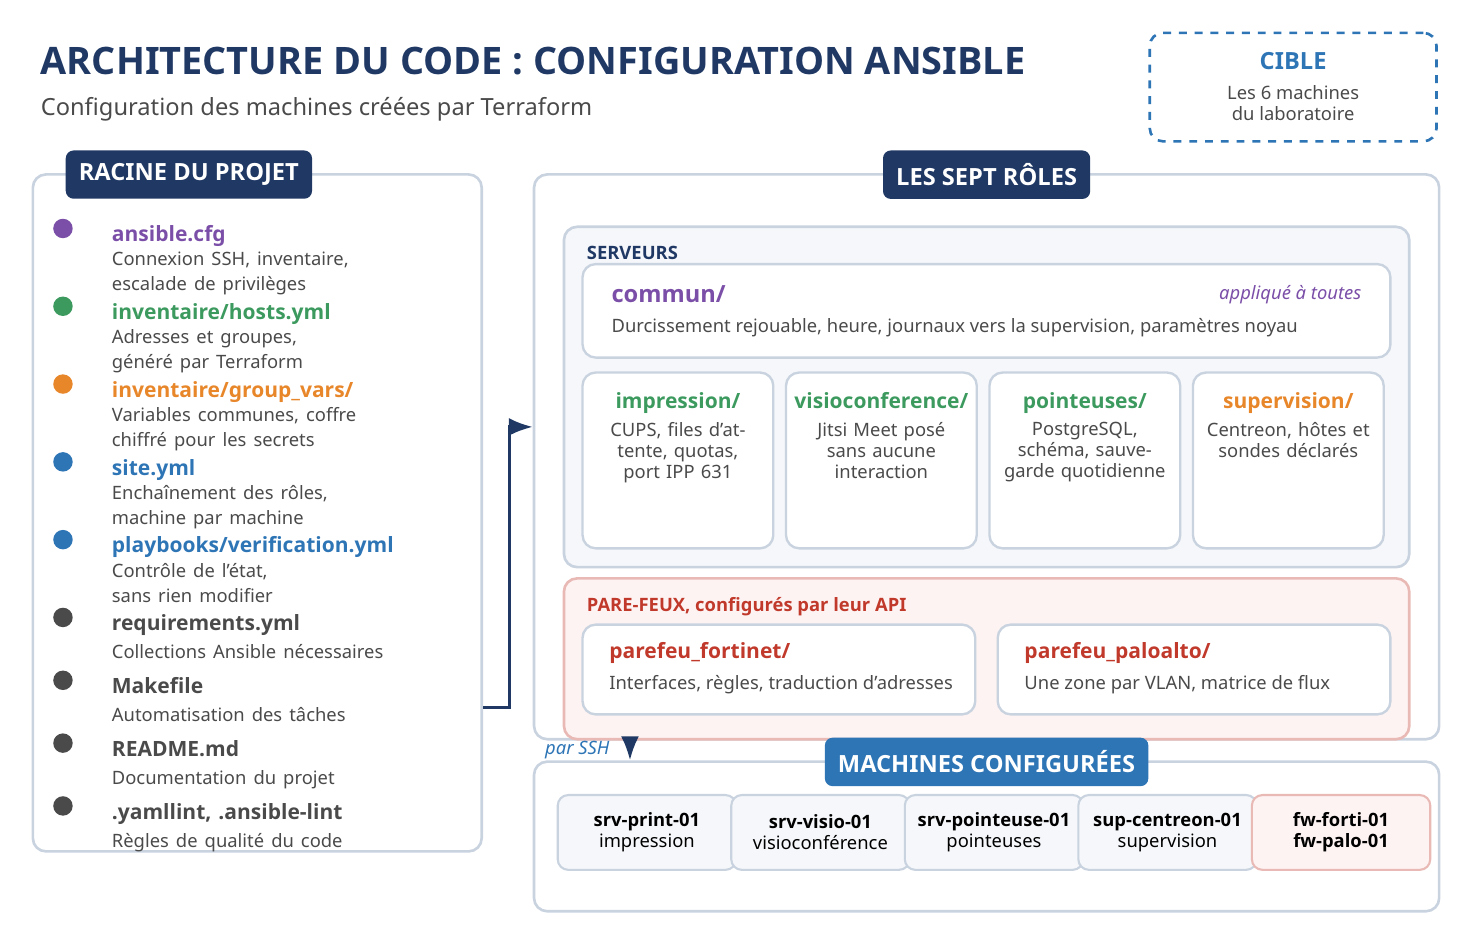
\includegraphics[width=\textwidth]{figures/figure3-ansible.png}
\caption{Architecture du code : configuration Ansible}
\end{figure}

\subsection{Les sept rôles}

\begin{table}[H]
\centering
\caption{Rôles Ansible et périmètre de chacun}
\begin{tabularx}{\textwidth}{L{3.4cm} L{3.4cm} Y}
\toprule
\rowcolor{soft}\textbf{Rôle} & \textbf{Machine} & \textbf{Ce qu'il fait} \\
\midrule
\ttb{commun} & toutes & Durcissement rejouable, heure, journaux vers la supervision, paramètres noyau \\
\ttb{impression} & \ttb{srv-print-01} & CUPS, files d'attente, quotas, accès limité au VLAN des postes \\
\ttb{visioconference} & \ttb{srv-visio-01} & Jitsi Meet installé sans aucune interaction \\
\ttb{pointeuses} & \ttb{srv-pointeuse-01} & PostgreSQL, schéma de collecte, sauvegarde quotidienne, contrôle de l'horloge \\
\ttb{supervision} & \ttb{sup-centreon-01} & Centreon, réception des journaux, déclaration des machines et des sondes \\
\ttb{parefeu\_fortinet} & \ttb{fw-forti-01} & Interfaces, règles, traduction d'adresses, export de la configuration \\
\ttb{parefeu\_paloalto} & \ttb{fw-palo-01} & Une zone et une sous-interface par VLAN, matrice de flux, profils \\
\bottomrule
\end{tabularx}
\end{table}

\subsection{Un inventaire généré, jamais écrit à la main}

Quand on sépare la création de l'infrastructure de sa configuration, une erreur
classique consiste à maintenir deux listes d'adresses, une par outil. Elles
finissent toujours par diverger.

Ici, le fichier \ttb{ansible/inventaire/hosts.yml} est \textbf{généré par
Terraform} à chaque déploiement, directement depuis \ttb{inventaire.tf}. Les
groupes sont déduits d'un champ porté par chaque machine. Ajouter un serveur
revient donc à ajouter une entrée dans l'inventaire Terraform : la machine est
créée, et Ansible sait immédiatement quel rôle lui appliquer.

Un pare-feu n'apparaît dans l'inventaire que si son image a été fournie. Tant
que ce n'est pas le cas, Ansible ne tente pas de le configurer.

\subsection{Le durcissement, mais rejouable}

Le durcissement demandé par \rid{INF-06} est posé par cloud-init à la création
de la machine, puis réaffirmé par le rôle \ttb{commun} à chaque exécution.

Cette redondance est volontaire. Cloud-init garantit qu'une machine neuve est
conforme ; le rôle \ttb{commun} garantit qu'elle l'est encore trois semaines
plus tard, même si quelqu'un a ouvert un port entre-temps. C'est ce qui permet
de prouver la conformité à tout moment, et non seulement le jour de la création.

\subsection{La supervision, qui satisfait réellement INF-04}

L'exigence \rid{INF-04} demande qu'une machine sous Centreon surveille toutes
les autres. Installer Centreon ne suffit donc pas : encore faut-il que les
machines y soient déclarées avec leurs sondes.

Le rôle procède en trois temps : installation depuis le dépôt officiel,
réception des journaux des autres machines, puis déclaration des hôtes et des
sondes par la ligne de commande Centreon plutôt que par l'interface web, afin
que l'opération reste rejouable. Les sondes dépendent du rôle de chaque machine
et reprennent le tableau des indicateurs du cahier des charges.

\subsection{Les pare-feux, en deux temps}

Les images FortiOS et PAN-OS n'acceptent pas cloud-init : ce sont des systèmes
constructeur fermés. La configuration se fait donc en deux étapes.

\textbf{L'amorçage}, une seule fois, rend la machine joignable et licenciée.
Palo Alto dispose d'un mécanisme officiel, un disque virtuel contenant
\ttb{init-cfg.txt} et \ttb{bootstrap.xml}. FortiGate accepte une configuration
déposée sur une image ISO attachée au premier démarrage.

\textbf{La configuration} passe ensuite par l'API du constructeur, autant de
fois qu'on le souhaite. Les collections \ttb{fortinet.fortios} et
\ttb{paloaltonetworks.panos} sont idempotentes : chaque exécution ramène le
pare-feu à l'état décrit dans les fichiers de variables. La configuration
obtenue est ensuite exportée dans le dépôt Git, ce qui répond à \rid{INF-08} et
\rid{INF-10}.

\begin{alertbox}[Limites de la licence d'évaluation Fortinet]
Elle plafonne la machine à trois interfaces, trois règles et trois routes. Le
rôle vérifie cette limite avant d'appliquer quoi que ce soit et s'arrête avec un
message clair si la configuration la dépasse, plutôt que de laisser l'API
échouer.
\end{alertbox}

\subsection{Gestion des secrets}

Aucun mot de passe ne figure en clair dans le dépôt. Les valeurs sensibles
vivent dans un fichier chiffré par \ttb{ansible-vault}, qui peut être versionné
sans risque. Seul le mot de passe du coffre ne l'est jamais.

%==============================================================================
\section{Vérifications réalisées}
%==============================================================================

Plusieurs contrôles ont été menés pour valider le code avant tout déploiement.

\begin{table}[H]
\centering
\caption{Contrôles effectués sur les deux couches}
\begin{tabularx}{\textwidth}{L{3.0cm} L{4.6cm} Y}
\toprule
\rowcolor{soft}\textbf{Couche} & \textbf{Contrôle} & \textbf{Résultat} \\
\midrule
Terraform & \ttb{terraform fmt} & Conforme \\
Terraform & \ttb{terraform validate} & Success! The configuration is valid. \\
Terraform & \ttb{terraform plan} & Va jusqu'au calcul des sorties, s'arrête uniquement faute de libvirt sur le poste actuel \\
Terraform & Rendu des cloud-init & YAML valide, 14 contrôles passés \\
Terraform & Inventaire & 6 machines conformes, 11 vCPU, 26 Go, 240 Go \\
\midrule
Ansible & \ttb{yamllint} & Conforme \\
Ansible & \ttb{ansible-playbook -{}-syntax-check} & Conforme \\
Ansible & \ttb{ansible-lint} & 0 échec, profil production, 5 étoiles sur 5 \\
Ansible & Lecture de l'inventaire & 6 groupes correctement construits \\
\midrule
Les deux & Cohérence croisée & 6 groupes déclarés, 7 rôles présents, aucun orphelin \\
\bottomrule
\end{tabularx}
\end{table}

L'analyse par \ttb{ansible-lint} a permis de corriger cinq points, dont
\textbf{deux véritables erreurs} qui auraient échoué à l'exécution : le module
\ttb{postgresql\_query} n'accepte pas le paramètre \ttb{path\_to\_script}, et le
module \ttb{panos\_ntp} n'existe pas dans la collection Palo Alto. Sans cette
analyse préalable, ces deux erreurs n'auraient été découvertes qu'en plein
déploiement sur la machine cible.

%==============================================================================
\section{Conformité aux exigences}
%==============================================================================

\begin{table}[H]
\centering
\caption{État des exigences INF-01 à INF-10}
\begin{tabularx}{\textwidth}{L{1.6cm} Y L{3.4cm}}
\toprule
\rowcolor{soft}\textbf{Réf.} & \textbf{Exigence} & \textbf{État} \\
\midrule
\rid{INF-02} & Une machine par service métier & \ok \\
\rid{INF-03} & Ubuntu Server 22.04 LTS & \ok \\
\rid{INF-04} & Centreon surveille toutes les machines & \ok, hôtes et sondes déclarés \\
\rid{INF-05} & Plan VLAN et adressage validés & \ok \\
\rid{INF-06} & Durcissement des serveurs & \ok, et rejouable \\
\rid{INF-07} & Heure synchronisée par NTP & \ok, serveurs et pare-feux \\
\rid{INF-08} & Configurations versionnées dans Git & \ok \\
\rid{INF-09} & Création automatisée par Terraform & \ok \\
\rid{INF-10} & Sauvegarde avant modification & \ok, export des pare-feux \\
\midrule
\rid{INF-01} & Deux pare-feux déployés & \textcolor{warn}{\textbf{Code prêt}}, images constructeur à fournir \\
\bottomrule
\end{tabularx}
\end{table}

%==============================================================================
\section{Ce qui reste à faire}
%==============================================================================

Trois points restent ouverts, et il est plus honnête de les poser clairement.

\textbf{Le code n'a pas encore tourné contre un véritable hyperviseur.} Il est
validé sur le plan syntaxique et cohérent d'un bout à l'autre, mais il n'a pas
été éprouvé à l'exécution. Le poste actuel est en Apple Silicon avec 16 Go de
mémoire, et libvirt n'y est pas disponible. Le premier déploiement réel se fera
sur la machine Intel fournie par l'entreprise.

\textbf{Les images des pare-feux restent à récupérer} auprès de Fortinet et de
Palo Alto. Tant qu'elles ne sont pas fournies, les serveurs se déploient
normalement et les pare-feux sont simplement absents de l'inventaire.

\textbf{Centreon s'arrêtera sur Ubuntu.} L'éditeur ne publie de dépôt que pour
Debian et la famille RHEL. Le rôle le détecte et s'arrête avec un message
expliquant la solution déjà prévue au cahier des charges : basculer cette seule
machine sous Debian 12.

%==============================================================================
\section{Conclusion}
%==============================================================================

L'infrastructure de la partie 1 est suffisamment avancée pour permettre un
déploiement reproductible sur la future machine Intel. Terraform couvre le
réseau, les machines virtuelles, l'adressage et l'amorçage. Ansible couvre
l'installation des services, la supervision et la configuration des deux
pare-feux.

Ce qui a changé récemment tient en trois points. Les services métiers ne sont
plus seulement préparés mais réellement installés et configurés. La supervision
déclare désormais les machines et leurs sondes, ce qui satisfait enfin
\rid{INF-04}. Enfin, les deux pare-feux disposent d'une configuration complète
et rejouable, là où il n'y avait auparavant que la création de la machine.

Les éléments qui restent manuels correspondent aux composants dont la
configuration dépend d'informations externes ou d'images constructeur : le
domaine et le certificat TLS de Jitsi, les images des pare-feux, et la
distribution attendue par Centreon.

L'objectif de la prochaine étape est de réaliser un déploiement complet sur la
machine cible, afin de valider l'ensemble de l'architecture en conditions
réelles.

\end{document}
